% -*- TeX-master: "../main.tex" -*-

\chapter{Arquitectura}
\label{sec:arquitectura}

En este capítulo se presenta la arquitectura general del intérprete
desarrollado para GPLC. Primero se expone el pipeline principal que
organiza el procesamiento de un programa, desde el código fuente hasta
una distribución simbólica de valores. Luego se describe la
organización modular del sistema y las interacciones entre sus
componentes. Finalmente, se presentan las estructuras de datos
fundamentales y las rutinas principales  que implementan la semántica del lenguaje.

\section{Pipeline principal}
El pipeline principal del intérprete se encuentra en el punto de
entrada de la aplicación, en el archivo \verb|main| del proyecto. Este pipeline actúa como un coordinador de las principales rutinas de la
aplicación, encargadas de ejecutar los pasos fundamentales del
pipeline descrito en la exposición del lenguaje GPLC.

La secuencia que describe los pasos de este pipeline se ilustra en la
figura  \ref{fig:pipeline}. A su vez, cada una de las rutinas que participan en este
procesamiento tiene acceso a abstracciones de las operaciones más
fundamentales, como las operaciones entre tipos y la satisfacibilidad de
fórmulas. La separación estricta de responsabilidades de cada módulo
permite mantener el desacoplamiento de las tareas y modelar con
claridad las fases de la formulación original del lenguaje.

\begin{figure}
  \centering
  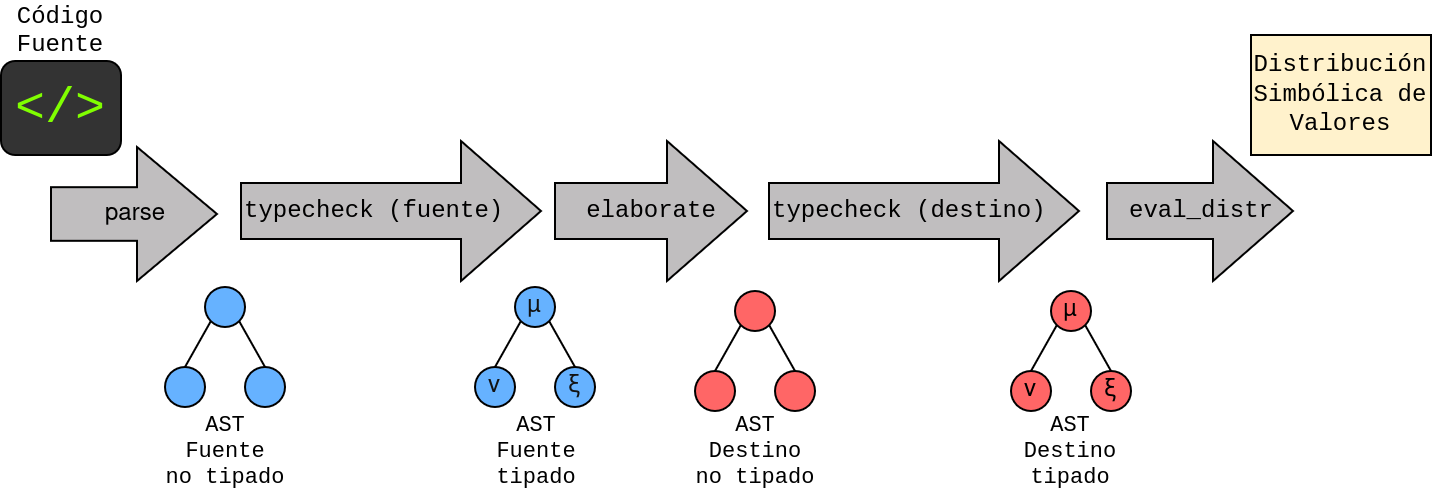
\includegraphics[width=\linewidth]{img/pipeline.png}
  \caption{Pipeline principal del intérprete.}
  \label{fig:pipeline}
\end{figure}



\section{Módulos y sus interacciones}

La figura \ref{fig:modulos} muestra la organización de los módulos y submódulos del intérprete. A continuación, se describe la responsabilidad principal de cada módulo.


\begin{figure}
  \centering
  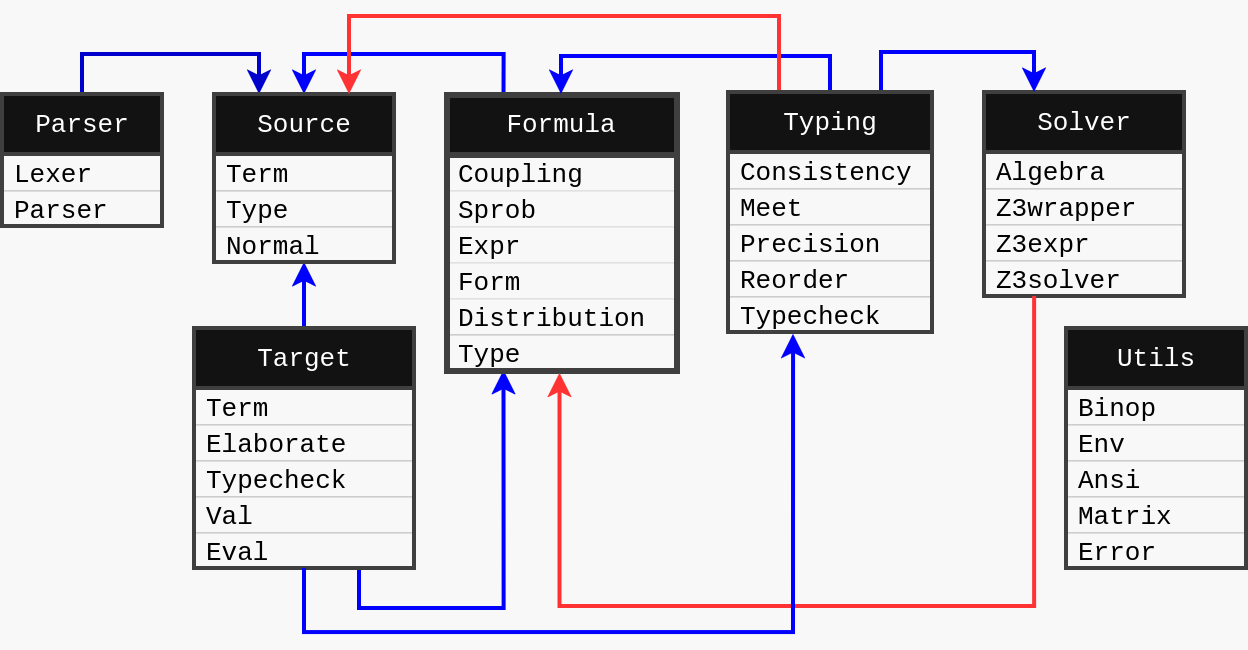
\includegraphics[width=0.8\linewidth]{img/dependency.png}
  \caption{Módulos y submódulos del intérprete.}
  \label{fig:modulos}
\end{figure}


\subsection{Parser} El módulo \verb|Parser| está encargado del procesamiento del archivo
con código fuente de GPLC. Sus dos submódulos \verb|Parser.Lexer| y
\verb|Parser.Parser| toman la responsabilidad de realizar los
análisis léxico y sintático de un programa, recibido por la entrada
estándar. El primer submódulo tiene como dependencia externa la
librería \verb|OCamllex|, un generador de analizadores
léxicos, y el segundo depende de la librería \verb|Menhir|, otra
librería robusta usada para la generación de analizadores sintáticos.
Como dependencia interna, el módulo \verb|Parser| depende del módulo
\verb|Source|, del cual obtiene las estructuras de datos y rutinas para
llevar a cabo la construcción del AST fuente no tipado.

\subsection{Source} El módulo \verb|Source| contiene todas las
estructuras de datos que constituyen el lenguaje fuente. Mientras que
\verb|Source.Type| define los tipos graduales simples y de
distribución y las probabilidades graduales, \verb|Source.Term| define la sintaxis abstracta de las expresiones del lenguaje fuente.

\subsection{Formula} El módulo \verb|Formula| es el responsable de
definir toda la infraestructura simbólica de la aplicación. En él,
el módulo \verb|Formula.Distribution| define qué es una distribución
simbólica, y tiene como dependencia \verb|Formula.Form| que define
las fórmulas que controlan las probabilidades de una distribución
simbólica. Este último submódulo depende a su vez de \verb|Formula.Expr|, que define el álgebra de las expresiones
que participan en las fórmulas. Finalmente, \verb|Formula.Expr| depende de \verb|Formula.Sprob| que es el módulo que define la probabilidad simbólica, la cual junto con los números participa en las expresiones que conforman las restricciones en las fórmulas. El submódulo \verb|Formula.Type| define los tipos de fórmula simples y de distribución, estos últimos usando la distribución simbólica paramétrica definida en \verb|Formula.Distribution| para implementar la distribución de tipos de fórmula simples. Adicionalmente, es el módulo \verb|Type| el que implementa la rutina para \emph{levantar} los tipos graduales a tipos de distribución.

\subsection{Solver} El módulo \verb|Solver| está a cargo de los
juicios de satisfacibilidad de las fórmulas definidas por el módulo
\verb|Formula|. El submódulo \verb|Solver.Algebra| define inductivamente
sus propias expresiones, similares a aquellas definidas por \verb|Formula.Expr|, e implementa transformaciones para convertir las fórmulas de \verb|Formula| a ecuaciones/inecuaciones nativas del módulo \verb|Solver.Algebra|. De este modo, un cambio de implementación solo implica una modificación de los transformadores, y no una modificación general del mecanismo de resolución. El submódulo \verb|Solver.Z3expr| utiliza los transformadores definidos en \verb|Solver.Z3wrapper| para traducir las ecuaciones e inecuaciones de \verb|Solver.Algebra| a expresiones nativas de la librería \verb|Z3|.
Para terminar, el submódulo \verb|Solver.Z3solver| contiene la función \verb|solve|, encargada de determinar la satisfacibilidad de una fórmula del módulo \verb|Formula|, la cual puede recibir directamente como argumento y transformar a expresión de Z3 gracias a las funcionalidades de transformación del módulo \verb|Solver|. De esta manera, \verb|solve| se constituye como el punto de integración del intérprete con Z3.


\subsection{Typing} El módulo \verb|Typing| es el encargado de la
definición de todas las operaciones entre tipos que se realizan en el
procesamiento del intérprete, y además implementa la rutina de chequeo
estático de tipos del lenguaje fuente. El submódulo \verb|Consistency|
implementa el juicio de consistencia para los tipos graduales en
\verb|Source.Type| y de fórmula en \verb|Formula.Type|. Los submódulos
\verb|Meet| y \verb|Precision| definen la operación de cómputo del
ínfimo y el juicio de precisión entre tipos de fórmula. Las
operaciones de consistencia, precisión e ínfimo hacen uso de las
estructuras que provee el módulo \verb|Formula.Coupling|, que modela
en función de las fórmulas de las distribuciones argumento, el sistema
de restricciones discutido en la sección \ref{par:symbolic},
retornando un sistema de restricciones cuya satisfacibilidad determina si
la operación del ínfimo está o no definida, o si los juicios de
consistencia y precisión son verdaderos o falsos. Las restricciones
provistas por \verb|Formula.Coupling| son resueltas en \verb|Z3|
mediante el pipeline descrito en el párrafo del módulo
\verb|Solver|. Finalmente, el submódulo \verb|Typecheck| es el que
realiza el proceso estático de tipado del AST fuente recibido del
módulo de \emph{parsing}.

\subsection{Target} En el módulo \verb|Target| se definen todas las
estructuras de datos y rutinas esenciales del lenguaje destino. El submódulo \verb|Term| define el AST del lenguaje destino. A diferencia
del módulo \verb|Source| que tiene un submódulo \verb|Type| donde define sus propios tipos (graduales), el módulo \verb|Target| deriva los suyos de \verb|Formula.Type|. \verb|Elaborate| es el submódulo a cargo de la elaboración (descrita en la sección \ref{sec:elab}), es decir, de la transformación del AST fuente tipado producido por \verb|Typing.Typecheck| a un AST destino no tipado cuya forma está definida por \verb|Term|. \verb|Typecheck| implementa el chequeo estático de tipos sobre el AST producido por la elaboración. El submódulo \verb|Val| define los valores crudos, valores y distribuciones de valores del lenguaje destino (descritos en la sección \ref{sec:target-language}). Finalmente, \verb|Eval| define la rutina que efectúa la evaluación del AST tipado, retornando una distribución simbólica de valores, con la forma definida en \verb|Val|.


\subsection{Resumen de dependencias}
Las dependencias entre módulos se muestran en la
figura~\ref{fig:modulos} mediante flechas, cuya punta indica el módulo
del cual se depende. Se omiten las dependencias asociadas a
\verb|Utils|, pues este módulo provee funcionalidades transversales a
todo el sistema.

En conjunto, estas dependencias reflejan la forma en que se organiza
el procesamiento de un programa dentro del intérprete. \verb|Parser|
depende de \verb|Source| para construir el AST fuente. \verb|Formula|
depende de \verb|Source| para hacer el \emph{levantamiento} de tipos
graduales a tipos de fórmula. \verb|Typing| depende de \verb|Source|
para tipar el AST fuente y operar sobre tipos graduales, de
\verb|Formula| para manipular tipos de fórmula, y de \verb|Solver|
para verificar la satisfacibilidad de las fórmulas involucradas. Por
su parte, \verb|Solver| depende de \verb|Formula| para traducir
fórmulas a expresiones nativas de Z3, mientras que \verb|Target|
depende de \verb|Source| para elaborar, a partir del AST fuente, el
AST destino, y de \verb|Typing| para ejecutar operaciones sobre tipos
de fórmula.




\section{Estructuras de datos}
En esta sección se presentan las estructuras de datos fundamentales del
intérprete. En particular, se describen los AST de los lenguajes fuente
y destino, los tipos graduales y los tipos de fórmula, y los entornos que permiten
asociar identificadores con tipos o valores en el proceso de tipado
y la evaluación.

\subsection{AST fuente}
El AST fuente es una estructura de datos implementada en el módulo
\verb|Source.Term|, y que modela la primera representación intermedia
del programa. Esta estructura tiene la flexibilidad adecuada al lugar
central que ocupa en la arquitectura de la aplicación, dado que
gracias a un parámetro de tipo, puede representar los AST no tipados
que produce la fase de \emph{parsing}, y luego representar los nodos
tipados con una anotación simple o de distribución, que devuelve el
chequeo estático efectuado por el módulo \verb|Typing.Typecheck|. El
AST fuente contiene además un objeto de metadatos, con la información
posicional de las expresiones del AST en el código fuente, lo cual es
fundamental para el reporte más útil de errores, mensajes de advertencia,
o un trabajo de depuración más informado.

\subsection{AST destino}
El AST destino está implementado en el módulo \verb|Target.Term|. Es
la estructura que constituye la segunda representación intermedia del
programa.  Tiene en común con su contraparte fuente el hecho de ser
una estructura paramétrica que se adapta tanto al requerimiento de
construir un AST no tipado (por ejemplo el que produce la fase
elaboración), como al de construir un AST con anotaciones de tipo (por
ejemplo, el que produce el chequeo estático del módulo
\verb|Target.Typecheck|). Al igual que el AST fuente, el AST destino
tiene un componente con metadatos, que en cada nodo preserva la
información posicional de cada nodo en el código fuente.


\subsection{Tipos graduales} Los tipos graduales
\verb|Source.Type.simple| y \verb|Source.Type.distr| modelan los tipos
usados en la sintaxis concreta del lenguaje. Por lo tanto, sus
constructores son usados en la fase de parsing para construir las
anotaciones (ascripciones) de tipo realizadas en el código fuente.
Forman parte integral de los nodos fuente, no solo en las sintaxis
abstracta de las ascripciones, sino también en la anotación de tipo en
cada nodo, hecha durante el chequeo estático. Las probabilidades
graduales no especificadas, también definidas en el módulo
\verb|Source.Type|, portan un identificador numérico
relevante para la arquitectura, pues una probabilidad desconocida se
propaga por la estructura del intérprete como una probabilidad
simbólica, y el identificador ayuda a asignar en distintas
instancias una misma variable para una probabilidad \verb|?|.

\subsection{Tipos de fórmula} Los tipos de fórmula
\verb|Formula.Type.simple| y \verb|Formula.Type.distr| modelan los
tipos usados exclusivamente en el lenguaje destino y en las
operaciones de tipo presentes en el módulo \verb|Typing|. El uso que
las operaciones de tipos hacen de estos está fundamentado en el poder
simbólico que le permite a las operaciones plantear el sistema de
restricciones descrito en la sección \ref{par:symbolic}. En el AST
destino, tanto las ascripciones (tipo ascrito y evidencia) como las
anotaciones por nodo realizadas en el chequeo estático utilizan tipos
de fórmula. Por último, estos tipos también son usados en el chequeo
dinámico de tipos de valores, efectuado en el módulo
\verb|Target.Eval|.

\subsection{Entornos} La última estructura de datos fundamental del
intérprete es el entorno, un mapa que permite
recuperar un objeto en función de un identificador. Las dos utilidades
que el entorno presta son {(1)} recuperar el tipo simple de una
variable durante los chequeos estáticos fuente
(\verb|Typing.Typecheck|) y destino (\verb|Target.Typecheck|), y
{(2)} recuperar el valor de una variable durante el proceso de
evaluación del AST tipado (\verb|Target.Eval|).

\section{Rutinas principales}

Las estructuras de datos descritas en la sección anterior son las
entradas y salidas de un conjunto de rutinas que, en el nivel más alto
del intérprete, representan las fases principales de procesamiento del
código fuente.

\subsection{Parsing} Esta rutina es la responsable de la
transformación del código fuente de un programa sintácticamente válido
de GPLC a un AST fuente no tipado, y de registrar en cada nodo que
construye la información posicional de inicio y término de la
expresión procesada.

\begin{center}
  \texttt{Código Fuente}
  $\rightarrow$
  \fbox{\texttt{parse}}
  $\rightarrow$
  \texttt{AST no tipado}
\end{center}


\subsection{Tipado fuente} Esta rutina del módulo \verb|Typing.Typecheck| recibe un AST fuente no tipado,
y retorna una estructura de la misma clase, pero con cada nodo portando un tipo simple o de distribución, inferido e insertado ahí por el chequeo estático de tipos. En esta rutina, se hace un uso recurrente  de \verb|Typing.Consistency| para verificar los juicios de consistencia propios del tipado gradual.
\begin{center}
  \texttt{AST Fuente no tipado}
  $\rightarrow$
  \fbox{\texttt{Typing.Typecheck.typecheck}}
  $\rightarrow$ \texttt{AST Fuente tipado}
\end{center}

\subsection{Elaboración} Esta transformación toma un AST fuente tipado, es decir, que cumple con el invariante de contener anotaciones de tipo en todos sus nodos, y transforma la expresión fuente en cada nodo a su expresión correspondiente en el lenguaje destino, retornando un AST destino no tipado. Sin embargo, la transformación también introduce explícitamente en el AST que construye, nuevas ascripciones con evidencia (además de las que introduce como traducción de las ascripciones del lenguaje fuente), por lo que el AST destino, en general, no tiene la misma estructura que el fuente. La elaboración depende
en gran parte de la operación \verb|Typing.Meet.meet| (ínfimo) para determinar las evidencias de casi todas las ascripciones que introduce en la nueva estructura. Esta fase preserva los metadatos de posición de cada nodo, propagando la información posicional hacia la ascripción que introduce para ese nodo.
\begin{center}
  \texttt{AST Fuente tipado}
  $\rightarrow$
  \fbox{\texttt{Target.Elaborate.elaborate}}
  $\rightarrow$
  \texttt{AST Destino no tipado}
\end{center}





\subsection{Tipado destino} Esta rutina verifica que después de la
elaboración el AST esté bien construido y siga cumpliendo con las reglas
estáticas de consistencia. Tras verificar las reglas de consistencia
establecidas para cada tipo de expresión, utilizando la consistencia
basada en evidencia (\verb|Precision.transitive_consistency_simple| y
\verb|Precision.transitive_consistency|), la rutina infiere un tipo
para cada nodo y lo anota en el espacio reservado en la estructura del
AST, retornando un AST destino tipado.  En el diseño de este
intérprete, la decisión de inferir el tipo de cada nodo destino y
anotarlo en el AST se fundamenta en el hecho de que una regla
central de la semántica operacional que reduce los programas a valores
--la reducción de la ascripción de distribución
$\eascr{\epsilon}{m}{\nu}$-- demanda conocer el tipo $\mu$ de la
subexpresión ascrita $m$, para definir la asignación de evidencias y
ascripciones simples a los valores de la distribución $\Vdistr$ a la
cual se evalúa $m$.
\begin{center}
  \texttt{AST Destino no tipado}
  $\rightarrow$
  \fbox{\texttt{Target.Typecheck.typecheck}}
  $\rightarrow$
  \texttt{AST Destino tipado}
\end{center}



\subsection{Evaluación}
Finalmente, en la fase de evaluación, la rutina
\verb|Target.Eval.eval_distr_value| toma el AST destino tipado, y
reduce cada uno de sus nodos a una distribución de valores. Las
distribuciones de valores de las subexpresiones se combinan de
distintas formas para llegar a producir una distribución simbólica de
valores, cuya fórmula es el resultado de la acumulación de las
fórmulas surgidas durante el proceso de evaluación. Si el programa
termina, la fórmula que restringe las variables de la distribución se
garantiza satisfacible.
\begin{center}
  \texttt{AST Destino Tipado}
  $\rightarrow$
  \fbox{\texttt{Target.Eval.eval\_distr\_value}}
  $\rightarrow$
  \texttt{Dis. simbólica de val.}
\end{center}


